\documentclass[12pt, final]{article}
\usepackage{fullpage,amsthm,amsfonts,amsmath}
\usepackage{enumerate}
\usepackage[margin=1in]{geometry}
\usepackage{color}
\usepackage{epsfig}
\usepackage{epstopdf}
\usepackage{datatool}
\usepackage{array}
\usepackage{tabu}
\usepackage{amsmath}
\usepackage{caption}
\usepackage{float}
\usepackage{tabularx, booktabs}
\usepackage{pdfpages}
\usepackage{standalone}
\usepackage{hyperref}
\usepackage{subfigure}
\usepackage{graphicx}
\hypersetup{colorlinks = true, urlcolor = blue, filecolor = blue, linkcolor = blue}
\floatstyle{plaintop}
\restylefloat{table}
\renewcommand{\thefootnote}{$\star$} 
\begin{document}
\title{Team 40: Predicting Mortality in ICU Setting (Project Draft).}

\date{\today}

%%
\renewcommand{\thefootnote}{$\dag$}
%%
\author{Vincent La\footnote{vincent.la@gatech.edu}, Avi Ananthakrishnan\footnote{avinash.ananthakrishnan@gatech.edu}}

\maketitle

\begin{abstract}
FILLER
\end{abstract} 

\newpage
%%%%%
\renewcommand{\thefootnote}{\number\value{footnote}} 
%%%%%
\section{Introduction} \label{Introduction}
Accurate knowledge of patient's clinical state is critical in a clinical setting. Patients in an intensive care unit are particularly in a critical state. Thus, if we can have better accurate mortality prediction within an ICU, we can use this to better understand which patients should be prioritized for clinical care and how we can better allocate resources. Within an ICU, there are many measurements being made from from various devices, but we know that there are both problems in terms of false positives and false negatives. While false negatives might seem to be more problematic, being too sensitive and introducing a lot of false positives also has problems as well. Too many false positives results in information fatigue and providers lose trust in signal as it's hard to separate from noise. By improving mortality prediction using data from EMRs and other clinically-relevant data, we can provide better predictions to improve efficiency and quality of care.

\section{Background and Literature Review}
\label{Background and Lit Review}
Siontis et. al (2011) \cite{Siontis} provide an empirical review of methodologies around mortality models. In this paper, the authors use Medline to identify studies published in 2009 that assessed AUC of predicting all cause mortality. What they find is that most studies at the time predicted mortality with modest accuracy, with large variability across populations, which makes sense since for since very high risk populations it may be easier to predict mortality, but for lower risk general populations, the class imbalance is very high with relatively few patients actually dying. A full list of the studies that the authors review and the approaches they use are documented in the paper (linked above). However, we also copy a portion of that table in Table \ref{Literature Review} as an illustrative example.
\\
\\
Taking a step back, we note that there have been many attempts to predict mortality, with some models being quite complicated. However, there have also been more technically simple models that attempt to predict mortality. For example, in DeSalvo et. al (2005) \cite{DeSalvo}, the authors attempt to predict mortality using a single question: ``In general, would you say your health is ... Excellent, Very Good, Good, Fair, or Poor". Similarly, we will provide a baseline model that only uses demographics and static variables (see Table \ref{Features} for the specific variables used) as features to predict mortality. While we know that we can do better using a richer feature set, doing a simple model with demographics and static variables provides us with a baseline to benchmark against.

\begin{table}[H]
\footnotesize
\newcolumntype{C}{>{\centering\arraybackslash}X}% centering
\caption{Literature Review}
\label{Literature Review}
\centering
\begin{tabularx}{\textwidth}{l C C}\hline
Disease Clinical Condition & Predictive Model & Variables Used \\ \hline
 &  &   \\
Cardiovascular Disease & Acute Kidney Injury Network (AKIN) & serum creatinine criteria or urine output criteria \\\
\\\
Critical Illness & Acute Myocardial Infarction in Switzerland (AMIS) model & age, Killip class, systolic blood pressure, heart rate, prehospital cardiopulmonary resuscitation, history of heart failure, history of cardiovascular disease \\\
\\\
Critical illness Gastroenterology-related & Acute Physiology And Chronic Health Evaluation (APACHE) II & temperature, mean arterial pressure, heart rate, respiratory rate, oxygenation or PaO2 , arterial pH, serum sodium, serum potassium, serum creatinine, hematocrit, white blood cell (WBC) count, Clasgow Coma Score\\\
\end{tabularx}
\end{table}

Next, there are a few papers that actually use the MIMIC III data for mortality prediction using ICU data. In Unfolding Physiological State: Mortality Model in Intensive Care Units, Ghassemi et. al (2014)\cite{Ghassemi}, the authors use Latent Variables Models to decompose free-text hospital notes into meaningful features to predict patient mortality. For the actual prediction, they use linear SVM in various setting (e.g. patient first arrives at hospital, In hospital mortality, 30 day mortality, etc.) and they largely find that using hospital notes improved AUCs.

\section{Methodology}
\label{Methodology}

What we will do in this project is to try to reproduce and improve models motivated by Unfolding Physiological State: Mortality Model in Intensive Care Units (Ghassemi et. al). In particular, what we find interesting is the use of free-text hospital notes to better predict mortality. This is because in many cases, there are already many mortality models, built both on Business Rules, and machine learning to predict mortality. Perhaps the biggest methodology to improve on existing mortality models is to use unstructured data, to see if there is any additional signal from notes and other text that we don't already get from structured data using EHRs.
\\
\\
To be more specific, we will use the same dataset as indicated in the Project guidelines, MIMIC III. This data set has ~45,000 patients, ~60,000 Hospital Admissions, ~200,000 Clinical notes, and ~6000 mortality events. We will then divide into 80\% training, 20\% test set. Similar to what is presented in the paper, we will first extract clinical baseline features, including age, sex, and SAPS-II score, from the database for every patient. We will then perform topic modeling, perhaps LDA, to do natural language processing on the notes to extract meaningful features. In terms of evaluating our model, we will predict on multiple iterations of the outcome variable, just as the paper does. For example, to evaluate 24 hour mortality predictions, in the training set, we will create a 24 hour prediction window and using the data that is transformed into features, we will measure AUC of mortality where outcome variable is mortality within 24 hours. We will then test on held-out test data set to report final test AUC.

\subsection{Data Exploration}
\label{Data Exploration}
The dataset contains 58,976 distinct hospital admissions with 46,520 distinct patients. Thus, most people in this dataset were admitted once, which makes sense, but there is also a long tail of readmissions.

\begin{figure}[H]
\centering
\caption{Admissions Distribution}
\label{AdmissionsDistribution}
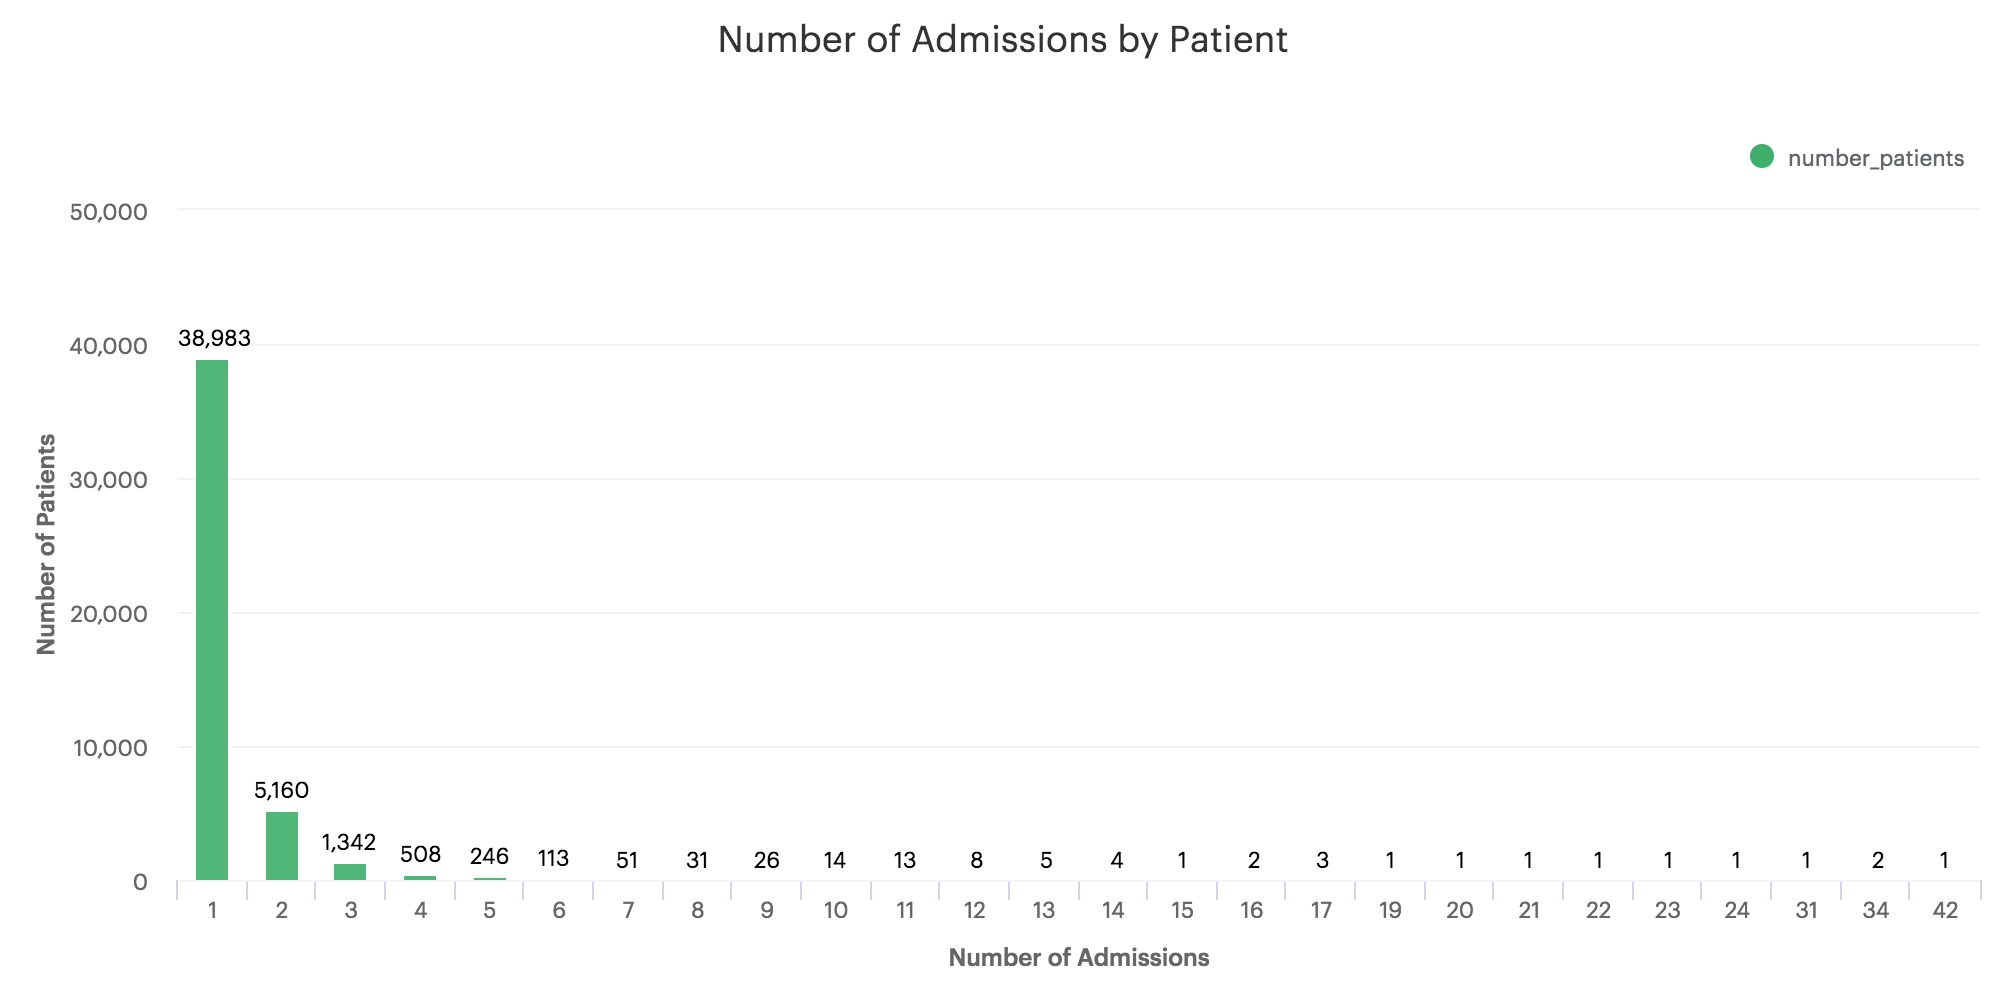
\includegraphics[page = {1}, scale = 0.4]{./images/admissions-distribution.png}
\end{figure}

About 39,000 patients were admitted once, with 5,160 admitted twice. However, there s a long tail of about 2,000 remaining patients who have been admitted more than twice in this time period, with the maximum being 42 admissions over this time period.
\\
\\
Furthermore, we note that admission lengths on average are about 10 days, but the median length of stay is closer to 6.5 days. This makes sense as again, the distribution is likely right skewed. There are patients with very long outlier lengths of stays dragging mean up, but the median, which is less sensitive to outliers is lower.

\begin{figure}[H]
\centering
\caption{Admissions Lengths (In Days)}
\label{AdmissionsLengths}
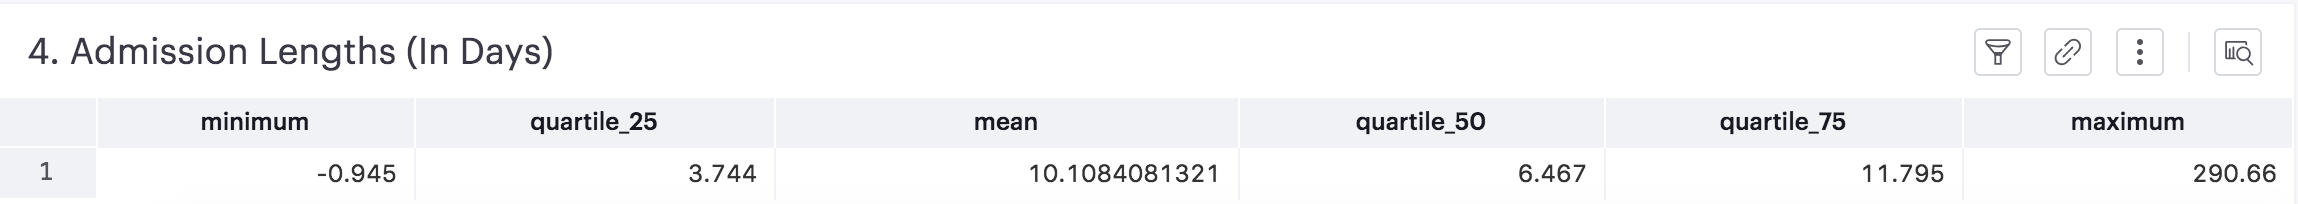
\includegraphics[page = {1}, scale = 0.4]{./images/admissions-lengths.png}
\end{figure}

Note that there are a few patients with negative lengths of stays. This is likely bad data. The longest a patient was in the hospital is about 290 days which is almost 10 months.
\\
\\
Next, we look at the breakdown of admissions by patients' insurance. This is interesting because the type of insurance a patient has is likely to be very correlated with patient characteristics. For example, Medicare patients will likely be older and have more acute risk. Medicaid is likely correlated with meaningful socioeconomic characteristics. As expected, many of the patients are Medicare patients, at about 48\% of the total population. This makes sense as Medicare patients are older and higher risk, so will comprise more of the admissions.

\begin{figure}[H]
\centering
\caption{Admissions by Patients' Insurance}
\label{AdmissionsByInsurance}
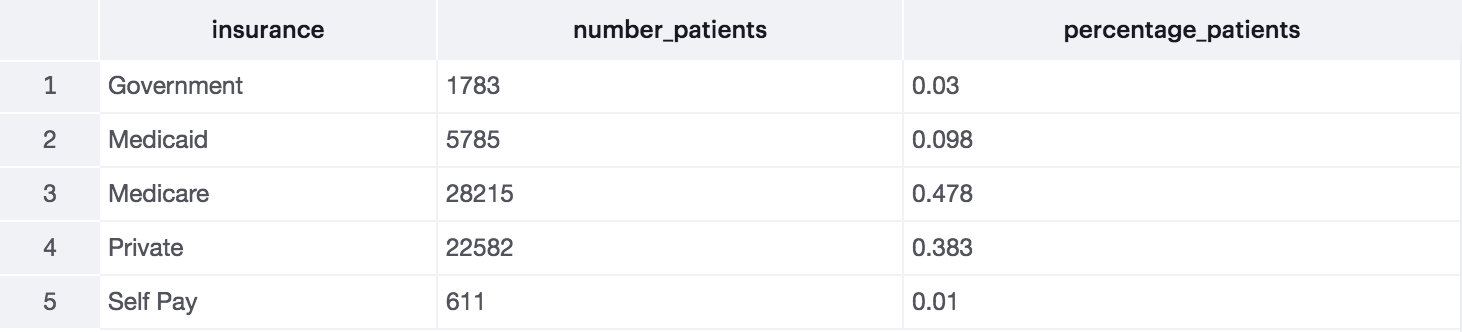
\includegraphics[page = {1}, scale = 0.4]{./images/admissions-insurance-summary.png}
\end{figure}

In addition, we note that about 5,800 patients are recorded as having died at some point after the admission.

\begin{figure}[H]
\centering
\caption{Admissions Deaths}
\label{AdmissionsDeaths}
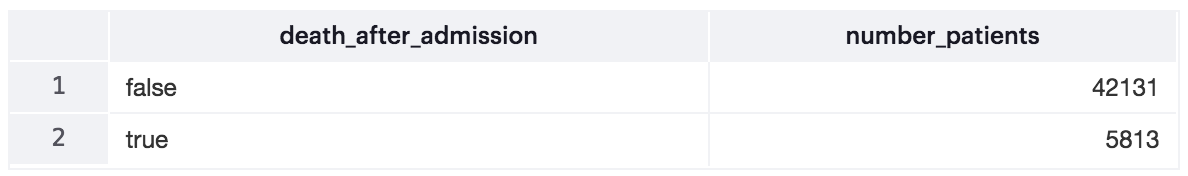
\includegraphics[page = {1}, scale = 0.4]{./images/admissions-deaths.png}
\end{figure}

In fact, if we look at the distribution of times to death, we see that the vast majority of deaths are recorded at the same time as the discharge time.

\begin{figure}[H]
\centering
\caption{Admissions Deaths Time Period}
\label{AdmissionsDeathsTimePeriod}
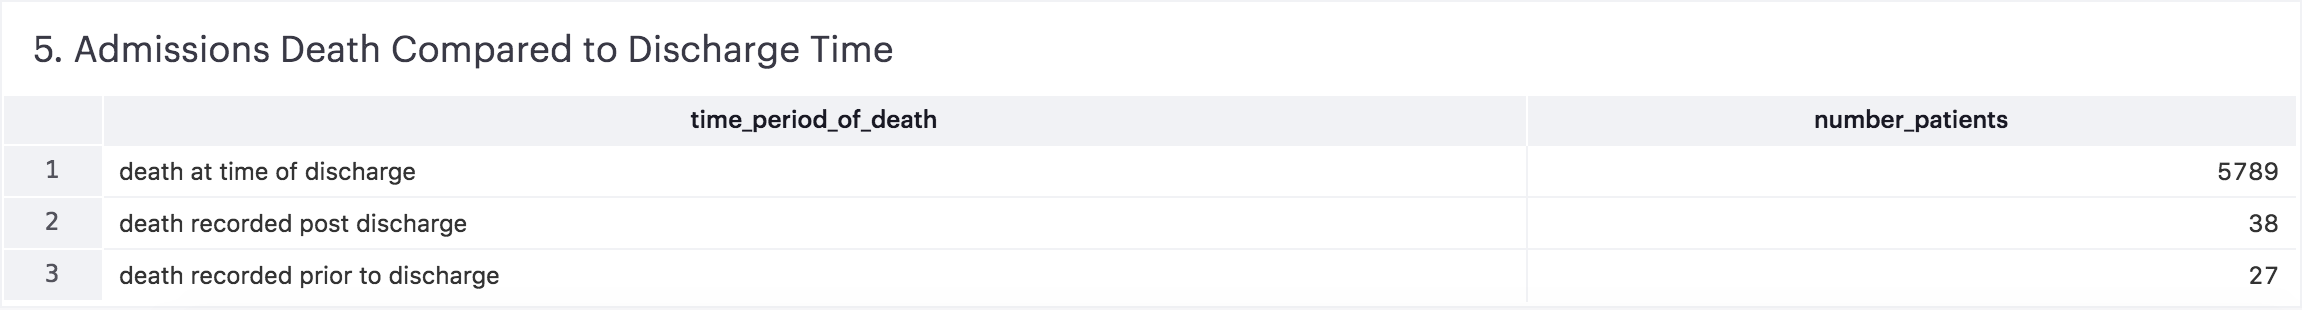
\includegraphics[page = {1}, scale = 0.4]{./images/admissions-deaths-time-period.png}
\end{figure}

Given this, it very likely means that mortalities recorded before the discharge time are due to clerical error. It's also possible that mortalities recorded after the discharge time are also a result of clerical error; although it is possible that the study followed up with the patient post-discharge.

\subsection{Feature Extraction}
Now that we have done some data exploration, this next section will discuss feature extraction and what features we actually used in our model to predict mortality.

\begin{table}[H]
\footnotesize
\newcolumntype{C}{>{\centering\arraybackslash}X}% centering
\caption{Features}
\label{Features}
\centering
\begin{tabularx}{\textwidth}{l C C}\hline
 & (1) & (2) \\\
Categories & Features & Extracted \\ \hline
 &  &   \\
Demographic and Static Features & Age, Gender, Ethnicity, Admission Type, Insurance Type &  \\\
\\\
Vital Signs & Heart Rate & Min, Max \\\
\end{tabularx}
\end{table}

\subsection{Model Architecture}
\label{Model Architecture}

\subsubsection{Baseline Model}
We first provide a baseline model that is a Random Forest model that only uses the Demographic and Static Features as described in Table \ref{Features}. The purpose of this is to provide a simple model that can serve as a baseline.

\section{Experimental Results}
\label{Experimental Results}

\subsubsection{Baseline Model}
We first show results of the baseline Random Forest model that only uses the Demographic and Static Features as described in Table \ref{Features}.

\begin{figure}[H]
\centering     %%% not \center
\subfigure[ROC]{\label{fig:a}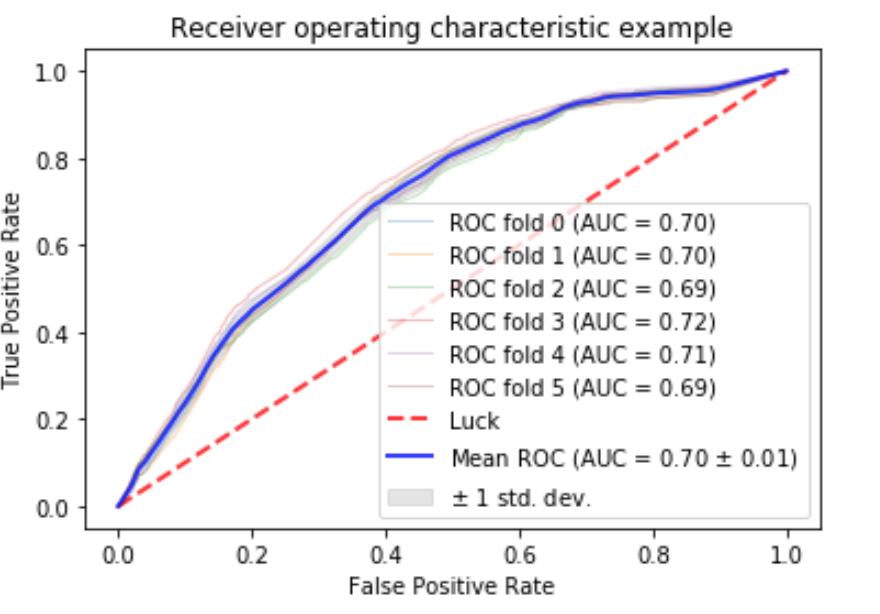
\includegraphics[width=70mm]{./images/modelperformance-baseline-roc}}
\subfigure[Precision Recall]{\label{fig:b}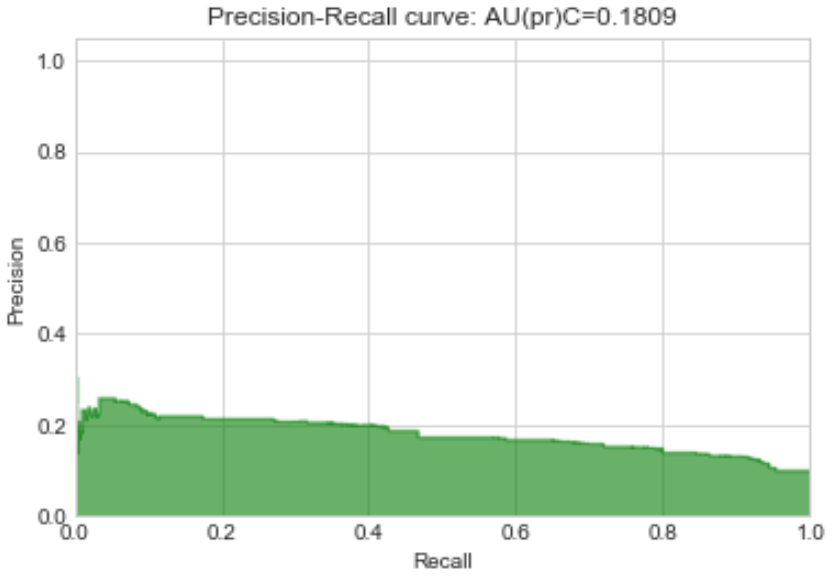
\includegraphics[width=70mm]{./images/modelperformance-baseline-pr}}
\caption{Baseline Model Performance}
\label{BaselineModelPerformance}
\end{figure}

As Figure \ref{BaselineModelPerformance} shows, even with just basic Demographic and Static Features, the model does OK. Average AUROC is about 0.70, and precision recall curve is about 0.1809 (with baseline mortality rate of about 9\% as we saw in Section \ref{Data Exploration}.

\section{Discussion}
\label{Discussion}

\section{Conclusion}
\label{Conclusion}
Filler

  \begin{thebibliography}{1}
    \bibitem{Afessa} Afessa B, Keegan MT. Predicting mortality in intensive care unit survivors using a subjective scoring system. Crit Care. 2007;11(1):109.   
    \bibitem{DeSalvo} DeSalvo KB, Fan VS, McDonell MB, Fihn SD. Predicting mortality and healthcare utilization with a single question. Health Serv Res. 2005;40(4):1234-46. 
    \bibitem{Ghassemi} Ghassemi M, Naumann T, Doshi-Velez F, et al. Unfolding Physiological State: Mortality Modelling in Intensive Care Units. KDD. 2014;2014:75-84.
    \bibitem{Johnson} Johnson AEW, Mark RG. Real-time mortality prediction in the Intensive Care Unit. AMIA Annu Symp Proc. 2018;2017:994-1003. Published 2018 Apr 16.
    \bibitem{Lipshutz} Lipshutz Angela KM, Feiner John R, Grimes Barbara, Gropper Michael A. Predicting mortality in the intensive care unit: a comparison of the University Health Consortium expected probability of mortality and the Mortality Prediction Model III. Journal of Intensive Care. 2016
    \bibitem{Silva} Silva I, Moody G, Scott DJ, Celi LA, Mark RG. Predicting In-Hospital Mortality of ICU Patients: The PhysioNet/Computing in Cardiology Challenge 2012. Comput Cardiol (2010). 2012;39:245-248.
	\bibitem{Siontis} Siontis GCM, Tzoulaki I, Ioannidis JPA. Predicting Death: An Empirical Evaluation of Predictive Tools for Mortality. Arch Intern Med. 2011;171(19):1721–1726. doi:10.1001/archinternmed.2011.334
	\bibitem{Teasdale} Teasdale Graham, Stocchetti Nino, Mass Andrew, Murray Gordon. Predicting Mortality in Critically Ill Patients. Critical Care Medicine. (2015). 2015;43:471-472
  
  \end{thebibliography}
\end{document}